\section{SYSTEM DEVELOPMENT}\label{sec:system-development}
\subsection{System development methodology}\label{subsec:implementation-and-ui-design}
The development of this project took an agile and iterative approach of system development. This was to ensure that any changes proposed by the users or feedback given by the users could be incorporated in the development of the project.  Scrum was used as a project management method where the project was divided into 8 weekly sprints. After every sprint, the development team could meet to track the progress of  the development and choose the tasks that needed to be done in the following sprint.  The team project leader was also the scrum master who was responsible for ensuring that the team was in constant communication with users for effective system development and also in-charge of the whole scrum process. 

The project underwent various iterations where after every iteration feedback was given. 
\subsection{System Architecture}\label{subsec:system architecture}
The system was developed using the client-server architecture as shown in Figure 6 in the Appendix. This was to ensure that the platform could be accessed remotely. During run time, the simulator and visualizer components of the system could connect with the MongoDB online server where the database operations were running on. 

The system is made up of 5 main components namely: system web view, internet measuring platforms, internet measurements collector, databases and the database server. System web view is the user interface of the system which contains both the simulator and the visualizer. The web view provides the user with the functionality to view and simulate the Africa internet topology. The internet measurements collector collects traceroute measurements from the internet measuring platforms namely: CAIDA, RIPE and Speedchecker. The collection component contains a python script which runs after every three hours and collects internet measurements from three measuring platforms. 

The database server has four components namely: data mapper, query manager, request handler and the response handler. The data mapper maps and structure the data collected in order to be stored in the databases. The query manager handles the various queries sent to the databases. The request and the response handlers manages the data requests and responses sent to and from web view to the databases.

The system has two databases namely: traceroute database and nodes and links database. The traceroute database stores the traceroute measurements from the different measuring platforms while the nodes and links database stores data on links and the nodes. Since to plot the internet topology nodes and links are needed, the traces stored in the traceroute database were used to model links and nodes. The modelled links and nodes were stored separately from the traces to ensure that when the client wants to visualize or simulate internet topology, nodes and links could be loaded faster. To allow flexibility of our database and higher availability, both databases that were developed are noSQL.  

\subsection{Class Diagram}
Three classes were developed namely: node, link and weighted graph. The class diagram in Figure 4 shows the classes and the relationships between them. The node class is responsible for storing information about the ASN and IXP. The information stored includes the node number, type of the node and the geographical position of the node.  The link class is responsible for storing information about links between the nodes. The information stored includes the source node, target node and the link delay. The weighted graph class is responsible for storing all information about the nodes and links. The weighted class implements the Dijkstra's algorithm which is used to determine the shortest route between two nodes. 
\begin{figure}[htp]
   \centering
     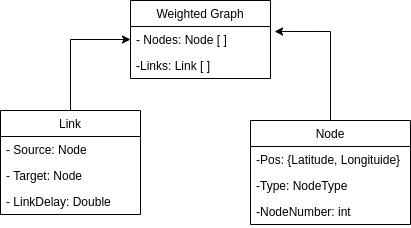
\includegraphics[width=8cm]{sections/pictures-diagrams/class-diagram.jpg}
   \caption{Class diagram for the system.}
    \label{figure:galaxy}
\end{figure}


\subsection{Framework and Technologies used}
The development of the system used various technologies in both front-end and the back-end. The python flask web framework was used to handle the front-end and back-end. The framework was used as it provided web tools and various python libraries which were necessary during the platform development which made the development easier as we could concentrate more on building the application rather than worrying how the dependencies will integrate. 

The web-view which forms the user interface was developed using HTML and CSS which are web markup and styling languages. JavaScript was used to script the functions that handled the events that occurred when various HTML components were clicked. To provide geographical mapping, the Google maps API was used for manipulating the Google Maps presented on the simulator. The D3 JavaScript library was also used to ensure good zooming and panning of the geographical maps. 

The back-end of the system was developed to run on the MongoDB online. MongoDB is a NoSQL online database which stores data in documents. This was necessary as we we dealt heavily with unstructured data that was collected from the internet measuring platforms. MongoDB also offers high availability of the data as it stores the data in three replicas ensuring that database queries can withstand fault tolerance. MongoDB also offers an option whereby you can connect the online database with a python application which made it easier for us to integrates the database with the rest of the application.  

The main python libraries that were used includes pymongo which was used to perform the database queries, geoIP2 database which was used to resolve the geo-location of a node given an IP address of the node, and the web-driver manager which is a library used to automate the management of web binaries. 

\subsection{System Testing}
System testing was done to evaluate whether the platform that was developed managed to achieve both functional and non-functional user requirements. The three types of testing that were carried are: usability testing, unit testing and functionality testing.
\subsubsection{Usability Testing}
10 users were selected to test the usability of the system. The users had background in networking and hence possible future users. During each test, users were asked to complete 5 uses cases using the simulator and answer if the simulator was useful and how easier it was to carry out the uses cases. 

"Add Node" and "Delete Node" use cases were the easiest as on average users took 1 minute to complete each tasks. The rest of the use cases took longer than 90 seconds to complete.

8 users agreed that the design of the simulator was okay but it needed improvement on three uses cases: "Add connection", "Remove connection" and "Simulate Traffic and View RTT". They pointed out the format of inputting the source and destination locations was not good enough. From this feedback, we enabled an information window when user clicks a node to allow them obtain the source and destination locations easily. 
\subsubsection{Unit and Integration Testing }
Unit testing was being carried out after every sprint to ensure that all units of source code were working well and properly. Since agile methodology was used to develop this project, testing was done regularly to ensure that any changes or issues that arose from source code could be addressed well in advance to avoid integration errors at the end of the project. During testing, the flask development environment was being changed from development to production to test how the system would behave during production.

During week 4 of the project, we experienced errors and bugs after testing due to data migration from local storage to the online MongoDB. This was due to failure of the flask environment to resolve the IP address of the remote database. This meant that the data storage unit of the system was not integrating well with our application. We decided to resolve the bug before proceeding to the next sprint and we managed to get a python library called dnspython which could integrate with pymongo to resolve the IP address of the remote MongoDB.  
\subsubsection{Functionality Testing}
Functionality testing was done to test if the developed system had fulfilled its functional requirements. Test cases for each use case were carried out as illustrated in the appendices. Test case for "Add IXP node" use case is illustrated in Figure 8. Test case for "Add Connection" use case is illustrated in Figure 9. Test case for "Delete node" use case is illustrated in Figure 10. Test case for "Delete Connection" use case is illustrated in Figure 11. Test case for "Simulate Traffic" and "View RTT" use cases illustrated in Figure 12. 
